\documentclass[1p]{elsarticle_modified}
%\bibliographystyle{elsarticle-num}

%\usepackage[colorlinks]{hyperref}
%\usepackage{abbrmath_seonhwa} %\Abb, \Ascr, \Acal ,\Abf, \Afrak
\usepackage{amsfonts}
\usepackage{amssymb}
\usepackage{amsmath}
\usepackage{amsthm}
\usepackage{scalefnt}
\usepackage{amsbsy}
\usepackage{kotex}
\usepackage{caption}
\usepackage{subfig}
\usepackage{color}
\usepackage{graphicx}
\usepackage{xcolor} %% white, black, red, green, blue, cyan, magenta, yellow
\usepackage{float}
\usepackage{setspace}
\usepackage{hyperref}

\usepackage{tikz}
\usetikzlibrary{arrows}

\usepackage{multirow}
\usepackage{array} % fixed length table
\usepackage{hhline}

%%%%%%%%%%%%%%%%%%%%%
\makeatletter
\renewcommand*\env@matrix[1][\arraystretch]{%
	\edef\arraystretch{#1}%
	\hskip -\arraycolsep
	\let\@ifnextchar\new@ifnextchar
	\array{*\c@MaxMatrixCols c}}
\makeatother %https://tex.stackexchange.com/questions/14071/how-can-i-increase-the-line-spacing-in-a-matrix
%%%%%%%%%%%%%%%

\usepackage[normalem]{ulem}

\newcommand{\msout}[1]{\ifmmode\text{\sout{\ensuremath{#1}}}\else\sout{#1}\fi}
%SOURCE: \msout is \stkout macro in https://tex.stackexchange.com/questions/20609/strikeout-in-math-mode

\newcommand{\cancel}[1]{
	\ifmmode
	{\color{red}\msout{#1}}
	\else
	{\color{red}\sout{#1}}
	\fi
}

\newcommand{\add}[1]{
	{\color{blue}\uwave{#1}}
}

\newcommand{\replace}[2]{
	\ifmmode
	{\color{red}\msout{#1}}{\color{blue}\uwave{#2}}
	\else
	{\color{red}\sout{#1}}{\color{blue}\uwave{#2}}
	\fi
}

\newcommand{\Sol}{\mathcal{S}} %segment
\newcommand{\D}{D} %diagram
\newcommand{\A}{\mathcal{A}} %arc


%%%%%%%%%%%%%%%%%%%%%%%%%%%%%5 test

\def\sl{\operatorname{\textup{SL}}(2,\Cbb)}
\def\psl{\operatorname{\textup{PSL}}(2,\Cbb)}
\def\quan{\mkern 1mu \triangleright \mkern 1mu}

\theoremstyle{definition}
\newtheorem{thm}{Theorem}[section]
\newtheorem{prop}[thm]{Proposition}
\newtheorem{lem}[thm]{Lemma}
\newtheorem{ques}[thm]{Question}
\newtheorem{cor}[thm]{Corollary}
\newtheorem{defn}[thm]{Definition}
\newtheorem{exam}[thm]{Example}
\newtheorem{rmk}[thm]{Remark}
\newtheorem{alg}[thm]{Algorithm}

\newcommand{\I}{\sqrt{-1}}
\begin{document}

%\begin{frontmatter}
%
%\title{Boundary parabolic representations of knots up to 8 crossings}
%
%%% Group authors per affiliation:
%\author{Yunhi Cho} 
%\address{Department of Mathematics, University of Seoul, Seoul, Korea}
%\ead{yhcho@uos.ac.kr}
%
%
%\author{Seonhwa Kim} %\fnref{s_kim}}
%\address{Center for Geometry and Physics, Institute for Basic Science, Pohang, 37673, Korea}
%\ead{ryeona17@ibs.re.kr}
%
%\author{Hyuk Kim}
%\address{Department of Mathematical Sciences, Seoul National University, Seoul 08826, Korea}
%\ead{hyukkim@snu.ac.kr}
%
%\author{Seokbeom Yoon}
%\address{Department of Mathematical Sciences, Seoul National University, Seoul, 08826,  Korea}
%\ead{sbyoon15@snu.ac.kr}
%
%\begin{abstract}
%We find all boundary parabolic representation of knots up to 8 crossings.
%
%\end{abstract}
%\begin{keyword}
%    \MSC[2010] 57M25 
%\end{keyword}
%
%\end{frontmatter}

%\linenumbers
%\tableofcontents
%
\newcommand\colored[1]{\textcolor{white}{\rule[-0.35ex]{0.8em}{1.4ex}}\kern-0.8em\color{red} #1}%
%\newcommand\colored[1]{\textcolor{white}{ #1}\kern-2.17ex	\textcolor{white}{ #1}\kern-1.81ex	\textcolor{white}{ #1}\kern-2.15ex\color{red}#1	}

{\Large $\underline{12a_{0281}~(K12a_{0281})}$}

\setlength{\tabcolsep}{10pt}
\renewcommand{\arraystretch}{1.6}
\vspace{1cm}\begin{tabular}{m{100pt}>{\centering\arraybackslash}m{274pt}}
\multirow{5}{120pt}{
	\centering
	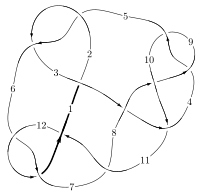
\includegraphics[width=112pt]{../../../GIT/diagram.site/Diagrams/png/1082_12a_0281.png}\\
\ \ \ A knot diagram\footnotemark}&
\allowdisplaybreaks
\textbf{Linearized knot diagam} \\
\cline{2-2}
 &
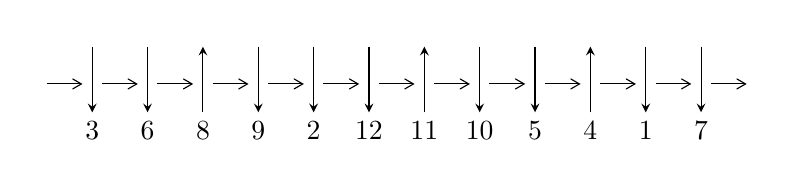
\begin{tikzpicture}[x=20pt, y=17pt]
	% nodes
	\node (C0) at (0, 0) {};
	\node (C1) at (1, 0) {};
	\node (C1U) at (1, +1) {};
	\node (C1D) at (1, -1) {3};

	\node (C2) at (2, 0) {};
	\node (C2U) at (2, +1) {};
	\node (C2D) at (2, -1) {6};

	\node (C3) at (3, 0) {};
	\node (C3U) at (3, +1) {};
	\node (C3D) at (3, -1) {8};

	\node (C4) at (4, 0) {};
	\node (C4U) at (4, +1) {};
	\node (C4D) at (4, -1) {9};

	\node (C5) at (5, 0) {};
	\node (C5U) at (5, +1) {};
	\node (C5D) at (5, -1) {2};

	\node (C6) at (6, 0) {};
	\node (C6U) at (6, +1) {};
	\node (C6D) at (6, -1) {12};

	\node (C7) at (7, 0) {};
	\node (C7U) at (7, +1) {};
	\node (C7D) at (7, -1) {11};

	\node (C8) at (8, 0) {};
	\node (C8U) at (8, +1) {};
	\node (C8D) at (8, -1) {10};

	\node (C9) at (9, 0) {};
	\node (C9U) at (9, +1) {};
	\node (C9D) at (9, -1) {5};

	\node (C10) at (10, 0) {};
	\node (C10U) at (10, +1) {};
	\node (C10D) at (10, -1) {4};

	\node (C11) at (11, 0) {};
	\node (C11U) at (11, +1) {};
	\node (C11D) at (11, -1) {1};

	\node (C12) at (12, 0) {};
	\node (C12U) at (12, +1) {};
	\node (C12D) at (12, -1) {7};
	\node (C13) at (13, 0) {};

	% arrows
	\draw[->,>={angle 60}]
	(C0) edge (C1) (C1) edge (C2) (C2) edge (C3) (C3) edge (C4) (C4) edge (C5) (C5) edge (C6) (C6) edge (C7) (C7) edge (C8) (C8) edge (C9) (C9) edge (C10) (C10) edge (C11) (C11) edge (C12) (C12) edge (C13) ;	\draw[->,>=stealth]
	(C1U) edge (C1D) (C2U) edge (C2D) (C3D) edge (C3U) (C4U) edge (C4D) (C5U) edge (C5D) (C6U) edge (C6D) (C7D) edge (C7U) (C8U) edge (C8D) (C9U) edge (C9D) (C10D) edge (C10U) (C11U) edge (C11D) (C12U) edge (C12D) ;
	\end{tikzpicture} \\
\hhline{~~} \\& 
\textbf{Solving Sequence} \\ \cline{2-2} 
 &
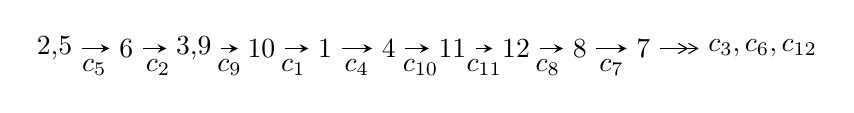
\begin{tikzpicture}[x=23pt, y=7pt]
	% node
	\node (A0) at (-1/8, 0) {2,5};
	\node (A1) at (1, 0) {6};
	\node (A2) at (33/16, 0) {3,9};
	\node (A3) at (25/8, 0) {10};
	\node (A4) at (33/8, 0) {1};
	\node (A5) at (41/8, 0) {4};
	\node (A6) at (49/8, 0) {11};
	\node (A7) at (57/8, 0) {12};
	\node (A8) at (65/8, 0) {8};
	\node (A9) at (73/8, 0) {7};
	\node (C1) at (1/2, -1) {$c_{5}$};
	\node (C2) at (3/2, -1) {$c_{2}$};
	\node (C3) at (21/8, -1) {$c_{9}$};
	\node (C4) at (29/8, -1) {$c_{1}$};
	\node (C5) at (37/8, -1) {$c_{4}$};
	\node (C6) at (45/8, -1) {$c_{10}$};
	\node (C7) at (53/8, -1) {$c_{11}$};
	\node (C8) at (61/8, -1) {$c_{8}$};
	\node (C9) at (69/8, -1) {$c_{7}$};
	\node (A10) at (11, 0) {$c_{3},c_{6},c_{12}$};

	% edge
	\draw[->,>=stealth]	
	(A0) edge (A1) (A1) edge (A2) (A2) edge (A3) (A3) edge (A4) (A4) edge (A5) (A5) edge (A6) (A6) edge (A7) (A7) edge (A8) (A8) edge (A9) ;
	\draw[->>,>={angle 60}]	
	(A9) edge (A10);
\end{tikzpicture} \\ 

\end{tabular} \\

\footnotetext{
The image of knot diagram is generated by the software ``\textbf{Draw programme}" developed by Andrew Bartholomew(\url{http://www.layer8.co.uk/maths/draw/index.htm\#Running-draw}), where we modified some parts for our purpose(\url{https://github.com/CATsTAILs/LinksPainter}).
}\phantom \\ \newline 
\centering \textbf{Ideals for irreducible components\footnotemark of $X_{\text{par}}$} 
 
\begin{align*}
I^u_{1}&=\langle 
5 u^{42}+12 u^{41}+\cdots+8 b-19,\;11 u^{42}+29 u^{41}+\cdots+8 a-44,\;u^{43}+u^{42}+\cdots+2 u+1\rangle \\
I^u_{2}&=\langle 
2.26163\times10^{32} u^{69}-1.52330\times10^{31} u^{68}+\cdots+1.91814\times10^{32} b+6.95419\times10^{32},\\
\phantom{I^u_{2}}&\phantom{= \langle  }-2.76673\times10^{33} u^{69}-1.62384\times10^{33} u^{68}+\cdots+9.59072\times10^{32} a-2.22275\times10^{34},\;u^{70}+u^{69}+\cdots+14 u+5\rangle \\
I^u_{3}&=\langle 
3 a^3+14 a^2+155 b-74 a-75,\;a^4-12 a^2+4 a+65,\;u-1\rangle \\
I^u_{4}&=\langle 
- a^2+b-3 a-2,\;a^3+3 a^2+3 a+1,\;u+1\rangle \\
\\
\end{align*}
\raggedright * 4 irreducible components of $\dim_{\mathbb{C}}=0$, with total 120 representations.\\
\footnotetext{All coefficients of polynomials are rational numbers. But the coefficients are sometimes approximated in decimal forms when there is not enough margin.}
\newpage
\renewcommand{\arraystretch}{1}
\centering \section*{I. $I^u_{1}= \langle 5 u^{42}+12 u^{41}+\cdots+8 b-19,\;11 u^{42}+29 u^{41}+\cdots+8 a-44,\;u^{43}+u^{42}+\cdots+2 u+1 \rangle$}
\flushleft \textbf{(i) Arc colorings}\\
\begin{tabular}{m{7pt} m{180pt} m{7pt} m{180pt} }
\flushright $a_{2}=$&$\begin{pmatrix}0\\u\end{pmatrix}$ \\
\flushright $a_{5}=$&$\begin{pmatrix}1\\0\end{pmatrix}$ \\
\flushright $a_{6}=$&$\begin{pmatrix}1\\u^2\end{pmatrix}$ \\
\flushright $a_{3}=$&$\begin{pmatrix}- u\\- u^3+u\end{pmatrix}$ \\
\flushright $a_{9}=$&$\begin{pmatrix}-1.37500 u^{42}-3.62500 u^{41}+\cdots+10.8750 u+5.50000\\-\frac{5}{8} u^{42}-\frac{3}{2} u^{41}+\cdots+\frac{37}{8} u+\frac{19}{8}\end{pmatrix}$ \\
\flushright $a_{10}=$&$\begin{pmatrix}-\frac{3}{4} u^{42}-\frac{17}{8} u^{41}+\cdots+\frac{25}{4} u+\frac{25}{8}\\-\frac{5}{8} u^{42}-\frac{3}{2} u^{41}+\cdots+\frac{37}{8} u+\frac{19}{8}\end{pmatrix}$ \\
\flushright $a_{1}=$&$\begin{pmatrix}u^3\\u^5- u^3+u\end{pmatrix}$ \\
\flushright $a_{4}=$&$\begin{pmatrix}\frac{1}{8} u^{42}+\frac{11}{8} u^{41}+\cdots-\frac{25}{8} u-\frac{3}{2}\\\frac{1}{8} u^{42}+\frac{5}{4} u^{41}+\cdots-\frac{15}{8} u-\frac{11}{8}\end{pmatrix}$ \\
\flushright $a_{11}=$&$\begin{pmatrix}-\frac{1}{8} u^{41}-\frac{1}{8} u^{40}+\cdots-\frac{3}{4} u+\frac{1}{8}\\-\frac{1}{8} u^{41}-\frac{1}{8} u^{40}+\cdots-\frac{3}{4} u+\frac{1}{8}\end{pmatrix}$ \\
\flushright $a_{12}=$&$\begin{pmatrix}-\frac{1}{8} u^{41}-\frac{1}{8} u^{40}+\cdots-\frac{3}{4} u+\frac{1}{8}\\-\frac{1}{8} u^{41}-\frac{1}{8} u^{40}+\cdots-\frac{3}{4} u+\frac{1}{8}\end{pmatrix}$ \\
\flushright $a_{8}=$&$\begin{pmatrix}\frac{1}{8} u^{42}+\frac{1}{8} u^{41}+\cdots-\frac{1}{8} u+1\\\frac{1}{8} u^{42}+\frac{1}{8} u^{41}+\cdots+\frac{3}{4} u^2-\frac{1}{8} u\end{pmatrix}$ \\
\flushright $a_{7}=$&$\begin{pmatrix}\frac{1}{8} u^{42}+\frac{1}{8} u^{41}+\cdots-\frac{1}{8} u+1\\\frac{1}{8} u^{42}+\frac{1}{8} u^{41}+\cdots+\frac{7}{4} u^2-\frac{1}{8} u\end{pmatrix}$\\&\end{tabular}
\flushleft \textbf{(ii) Obstruction class $= -1$}\\~\\
\flushleft \textbf{(iii) Cusp Shapes $= -\frac{7}{2} u^{42}-\frac{19}{4} u^{41}+\cdots-\frac{1}{2} u-\frac{49}{4}$}\\~\\
\newpage\renewcommand{\arraystretch}{1}
\flushleft \textbf{(iv) u-Polynomials at the component}\newline \\
\begin{tabular}{m{50pt}|m{274pt}}
Crossings & \hspace{64pt}u-Polynomials at each crossing \\
\hline $$\begin{aligned}c_{1},c_{11}\end{aligned}$$&$\begin{aligned}
&u^{43}+21 u^{42}+\cdots+10 u+1
\end{aligned}$\\
\hline $$\begin{aligned}c_{2},c_{5},c_{6}\\c_{12}\end{aligned}$$&$\begin{aligned}
&u^{43}+u^{42}+\cdots+2 u+1
\end{aligned}$\\
\hline $$\begin{aligned}c_{3}\end{aligned}$$&$\begin{aligned}
&u^{43}+3 u^{42}+\cdots+238 u+194
\end{aligned}$\\
\hline $$\begin{aligned}c_{4},c_{9}\end{aligned}$$&$\begin{aligned}
&u^{43}-3 u^{42}+\cdots-6 u+2
\end{aligned}$\\
\hline $$\begin{aligned}c_{7}\end{aligned}$$&$\begin{aligned}
&u^{43}+3 u^{42}+\cdots+256 u+256
\end{aligned}$\\
\hline $$\begin{aligned}c_{8}\end{aligned}$$&$\begin{aligned}
&u^{43}+21 u^{42}+\cdots+4 u+4
\end{aligned}$\\
\hline $$\begin{aligned}c_{10}\end{aligned}$$&$\begin{aligned}
&u^{43}-9 u^{42}+\cdots-118 u+38
\end{aligned}$\\
\hline
\end{tabular}\\~\\
\newpage\renewcommand{\arraystretch}{1}
\flushleft \textbf{(v) Riley Polynomials at the component}\newline \\
\begin{tabular}{m{50pt}|m{274pt}}
Crossings & \hspace{64pt}Riley Polynomials at each crossing \\
\hline $$\begin{aligned}c_{1},c_{11}\end{aligned}$$&$\begin{aligned}
&y^{43}+11 y^{42}+\cdots+18 y-1
\end{aligned}$\\
\hline $$\begin{aligned}c_{2},c_{5},c_{6}\\c_{12}\end{aligned}$$&$\begin{aligned}
&y^{43}-21 y^{42}+\cdots+10 y-1
\end{aligned}$\\
\hline $$\begin{aligned}c_{3}\end{aligned}$$&$\begin{aligned}
&y^{43}+3 y^{42}+\cdots+106308 y-37636
\end{aligned}$\\
\hline $$\begin{aligned}c_{4},c_{9}\end{aligned}$$&$\begin{aligned}
&y^{43}-21 y^{42}+\cdots+4 y-4
\end{aligned}$\\
\hline $$\begin{aligned}c_{7}\end{aligned}$$&$\begin{aligned}
&y^{43}+23 y^{42}+\cdots+1441792 y-65536
\end{aligned}$\\
\hline $$\begin{aligned}c_{8}\end{aligned}$$&$\begin{aligned}
&y^{43}+3 y^{42}+\cdots+80 y-16
\end{aligned}$\\
\hline $$\begin{aligned}c_{10}\end{aligned}$$&$\begin{aligned}
&y^{43}+15 y^{42}+\cdots-31068 y-1444
\end{aligned}$\\
\hline
\end{tabular}\\~\\
\newpage\flushleft \textbf{(vi) Complex Volumes and Cusp Shapes}
$$\begin{array}{c|c|c}  
\text{Solutions to }I^u_{1}& \I (\text{vol} + \sqrt{-1}CS) & \text{Cusp shape}\\
 \hline 
\begin{aligned}
u &= -0.748644 + 0.637641 I \\
a &= \phantom{-}0.080537 - 0.526871 I \\
b &= \phantom{-}1.013350 + 0.562622 I\end{aligned}
 & \phantom{-}1.89821 - 0.96458 I & -3.28074 - 0.62200 I \\ \hline\begin{aligned}
u &= -0.748644 - 0.637641 I \\
a &= \phantom{-}0.080537 + 0.526871 I \\
b &= \phantom{-}1.013350 - 0.562622 I\end{aligned}
 & \phantom{-}1.89821 + 0.96458 I & -3.28074 + 0.62200 I \\ \hline\begin{aligned}
u &= \phantom{-}0.804750 + 0.623565 I \\
a &= \phantom{-}0.222175 - 1.018610 I \\
b &= \phantom{-}0.529140 + 0.662060 I\end{aligned}
 & \phantom{-}3.32140 - 3.80226 I & -0.99469 + 6.39942 I \\ \hline\begin{aligned}
u &= \phantom{-}0.804750 - 0.623565 I \\
a &= \phantom{-}0.222175 + 1.018610 I \\
b &= \phantom{-}0.529140 - 0.662060 I\end{aligned}
 & \phantom{-}3.32140 + 3.80226 I & -0.99469 - 6.39942 I \\ \hline\begin{aligned}
u &= -0.900705 + 0.522951 I \\
a &= -1.36239 - 0.90089 I \\
b &= -1.035780 - 0.144530 I\end{aligned}
 & -1.80687 + 4.07167 I & -9.95788 - 6.11472 I \\ \hline\begin{aligned}
u &= -0.900705 - 0.522951 I \\
a &= -1.36239 + 0.90089 I \\
b &= -1.035780 + 0.144530 I\end{aligned}
 & -1.80687 - 4.07167 I & -9.95788 + 6.11472 I \\ \hline\begin{aligned}
u &= \phantom{-}0.894694 + 0.620124 I \\
a &= -0.903919 - 0.027255 I \\
b &= \phantom{-}0.412108 - 0.716509 I\end{aligned}
 & \phantom{-}2.75595 - 5.96538 I & -2.44764 + 6.68032 I \\ \hline\begin{aligned}
u &= \phantom{-}0.894694 - 0.620124 I \\
a &= -0.903919 + 0.027255 I \\
b &= \phantom{-}0.412108 + 0.716509 I\end{aligned}
 & \phantom{-}2.75595 + 5.96538 I & -2.44764 - 6.68032 I \\ \hline\begin{aligned}
u &= -0.929214 + 0.629305 I \\
a &= \phantom{-}1.48748 + 2.03173 I \\
b &= \phantom{-}1.082430 - 0.572492 I\end{aligned}
 & \phantom{-}0.79286 + 10.89690 I & -5.90232 - 10.97141 I \\ \hline\begin{aligned}
u &= -0.929214 - 0.629305 I \\
a &= \phantom{-}1.48748 - 2.03173 I \\
b &= \phantom{-}1.082430 + 0.572492 I\end{aligned}
 & \phantom{-}0.79286 - 10.89690 I & -5.90232 + 10.97141 I\\
 \hline 
 \end{array}$$\newpage$$\begin{array}{c|c|c}  
\text{Solutions to }I^u_{1}& \I (\text{vol} + \sqrt{-1}CS) & \text{Cusp shape}\\
 \hline 
\begin{aligned}
u &= \phantom{-}0.821297 + 0.283255 I \\
a &= -2.93341 + 0.45122 I \\
b &= -1.139100 - 0.422179 I\end{aligned}
 & -4.79407 - 5.18096 I & -10.28186 + 9.63354 I \\ \hline\begin{aligned}
u &= \phantom{-}0.821297 - 0.283255 I \\
a &= -2.93341 - 0.45122 I \\
b &= -1.139100 + 0.422179 I\end{aligned}
 & -4.79407 + 5.18096 I & -10.28186 - 9.63354 I \\ \hline\begin{aligned}
u &= -0.230146 + 0.788552 I \\
a &= -1.13253 + 1.42685 I \\
b &= -1.118980 - 0.552972 I\end{aligned}
 & -0.99153 - 7.44962 I & -4.80788 + 5.14749 I \\ \hline\begin{aligned}
u &= -0.230146 - 0.788552 I \\
a &= -1.13253 - 1.42685 I \\
b &= -1.118980 + 0.552972 I\end{aligned}
 & -0.99153 + 7.44962 I & -4.80788 - 5.14749 I \\ \hline\begin{aligned}
u &= -0.469810 + 0.644333 I \\
a &= -0.302237 - 1.339690 I \\
b &= -0.975090 + 0.534458 I\end{aligned}
 & \phantom{-}1.37306 + 3.64200 I & -1.97274 - 6.09907 I \\ \hline\begin{aligned}
u &= -0.469810 - 0.644333 I \\
a &= -0.302237 + 1.339690 I \\
b &= -0.975090 - 0.534458 I\end{aligned}
 & \phantom{-}1.37306 - 3.64200 I & -1.97274 + 6.09907 I \\ \hline\begin{aligned}
u &= \phantom{-}0.766243 + 0.202401 I \\
a &= \phantom{-}2.75313 - 0.25431 I \\
b &= \phantom{-}1.137770 - 0.456668 I\end{aligned}
 & -4.56135 + 2.74808 I & -8.63761 + 1.53004 I \\ \hline\begin{aligned}
u &= \phantom{-}0.766243 - 0.202401 I \\
a &= \phantom{-}2.75313 + 0.25431 I \\
b &= \phantom{-}1.137770 + 0.456668 I\end{aligned}
 & -4.56135 - 2.74808 I & -8.63761 - 1.53004 I \\ \hline\begin{aligned}
u &= -0.735504 + 0.278747 I \\
a &= \phantom{-}0.282174 - 0.733558 I \\
b &= \phantom{-}0.039236 - 0.647029 I\end{aligned}
 & -1.56483 + 1.33884 I & -5.91775 - 5.05918 I \\ \hline\begin{aligned}
u &= -0.735504 - 0.278747 I \\
a &= \phantom{-}0.282174 + 0.733558 I \\
b &= \phantom{-}0.039236 + 0.647029 I\end{aligned}
 & -1.56483 - 1.33884 I & -5.91775 + 5.05918 I\\
 \hline 
 \end{array}$$\newpage$$\begin{array}{c|c|c}  
\text{Solutions to }I^u_{1}& \I (\text{vol} + \sqrt{-1}CS) & \text{Cusp shape}\\
 \hline 
\begin{aligned}
u &= \phantom{-}0.244913 + 0.744578 I \\
a &= \phantom{-}0.531179 + 0.238214 I \\
b &= -0.323354 - 0.721542 I\end{aligned}
 & \phantom{-}1.32443 + 2.58910 I & -1.27516 - 1.34286 I \\ \hline\begin{aligned}
u &= \phantom{-}0.244913 - 0.744578 I \\
a &= \phantom{-}0.531179 - 0.238214 I \\
b &= -0.323354 + 0.721542 I\end{aligned}
 & \phantom{-}1.32443 - 2.58910 I & -1.27516 + 1.34286 I \\ \hline\begin{aligned}
u &= \phantom{-}1.156160 + 0.436646 I \\
a &= -2.27777 + 0.12084 I \\
b &= -1.157530 + 0.522173 I\end{aligned}
 & -8.54240 + 0.05443 I & -13.25807 + 1.27713 I \\ \hline\begin{aligned}
u &= \phantom{-}1.156160 - 0.436646 I \\
a &= -2.27777 - 0.12084 I \\
b &= -1.157530 - 0.522173 I\end{aligned}
 & -8.54240 - 0.05443 I & -13.25807 - 1.27713 I \\ \hline\begin{aligned}
u &= -1.151630 + 0.457340 I \\
a &= -0.353184 + 0.596905 I \\
b &= -0.199663 + 0.761913 I\end{aligned}
 & -5.75226 + 4.72408 I & -9.80399 - 4.71758 I \\ \hline\begin{aligned}
u &= -1.151630 - 0.457340 I \\
a &= -0.353184 - 0.596905 I \\
b &= -0.199663 - 0.761913 I\end{aligned}
 & -5.75226 - 4.72408 I & -9.80399 + 4.71758 I \\ \hline\begin{aligned}
u &= \phantom{-}0.368859 + 0.661669 I \\
a &= \phantom{-}0.306430 - 0.852800 I \\
b &= -0.587313 + 0.602075 I\end{aligned}
 & \phantom{-}2.51319 + 0.87621 I & \phantom{-}0.614769 - 0.778636 I \\ \hline\begin{aligned}
u &= \phantom{-}0.368859 - 0.661669 I \\
a &= \phantom{-}0.306430 + 0.852800 I \\
b &= -0.587313 - 0.602075 I\end{aligned}
 & \phantom{-}2.51319 - 0.87621 I & \phantom{-}0.614769 + 0.778636 I \\ \hline\begin{aligned}
u &= -1.139070 + 0.530786 I \\
a &= -0.355456 - 0.234216 I \\
b &= -0.851539 - 0.591728 I\end{aligned}
 & -2.78091 + 5.63282 I & -7.68461 - 3.26690 I \\ \hline\begin{aligned}
u &= -1.139070 - 0.530786 I \\
a &= -0.355456 + 0.234216 I \\
b &= -0.851539 + 0.591728 I\end{aligned}
 & -2.78091 - 5.63282 I & -7.68461 + 3.26690 I\\
 \hline 
 \end{array}$$\newpage$$\begin{array}{c|c|c}  
\text{Solutions to }I^u_{1}& \I (\text{vol} + \sqrt{-1}CS) & \text{Cusp shape}\\
 \hline 
\begin{aligned}
u &= -0.140641 + 0.728292 I \\
a &= \phantom{-}1.221290 - 0.180259 I \\
b &= \phantom{-}1.104910 - 0.276140 I\end{aligned}
 & -2.87123 + 0.12831 I & -7.71481 - 0.77840 I \\ \hline\begin{aligned}
u &= -0.140641 - 0.728292 I \\
a &= \phantom{-}1.221290 + 0.180259 I \\
b &= \phantom{-}1.104910 + 0.276140 I\end{aligned}
 & -2.87123 - 0.12831 I & -7.71481 + 0.77840 I \\ \hline\begin{aligned}
u &= \phantom{-}1.178850 + 0.464753 I \\
a &= \phantom{-}2.75499 - 0.42952 I \\
b &= \phantom{-}1.173340 + 0.326229 I\end{aligned}
 & -9.87566 - 8.22613 I & -14.9046 + 7.3441 I \\ \hline\begin{aligned}
u &= \phantom{-}1.178850 - 0.464753 I \\
a &= \phantom{-}2.75499 + 0.42952 I \\
b &= \phantom{-}1.173340 - 0.326229 I\end{aligned}
 & -9.87566 + 8.22613 I & -14.9046 - 7.3441 I \\ \hline\begin{aligned}
u &= \phantom{-}1.165570 + 0.544375 I \\
a &= -1.09575 + 0.95090 I \\
b &= -0.701705 - 0.646518 I\end{aligned}
 & -2.33002 - 10.45450 I & -6.00000 + 9.18893 I \\ \hline\begin{aligned}
u &= \phantom{-}1.165570 - 0.544375 I \\
a &= -1.09575 - 0.95090 I \\
b &= -0.701705 + 0.646518 I\end{aligned}
 & -2.33002 + 10.45450 I & -6.00000 - 9.18893 I \\ \hline\begin{aligned}
u &= -1.206960 + 0.526147 I \\
a &= \phantom{-}2.05937 + 1.28523 I \\
b &= \phantom{-}1.169220 + 0.252610 I\end{aligned}
 & -8.97242 + 9.46345 I & -14.0760 - 5.8340 I \\ \hline\begin{aligned}
u &= -1.206960 - 0.526147 I \\
a &= \phantom{-}2.05937 - 1.28523 I \\
b &= \phantom{-}1.169220 - 0.252610 I\end{aligned}
 & -8.97242 - 9.46345 I & -14.0760 + 5.8340 I \\ \hline\begin{aligned}
u &= \phantom{-}1.203670 + 0.545583 I \\
a &= \phantom{-}0.839018 + 0.724019 I \\
b &= -0.298947 + 0.789061 I\end{aligned}
 & -4.36938 - 12.53960 I & -6.00000 + 7.94110 I \\ \hline\begin{aligned}
u &= \phantom{-}1.203670 - 0.545583 I \\
a &= \phantom{-}0.839018 - 0.724019 I \\
b &= -0.298947 - 0.789061 I\end{aligned}
 & -4.36938 + 12.53960 I & -6.00000 - 7.94110 I\\
 \hline 
 \end{array}$$\newpage$$\begin{array}{c|c|c}  
\text{Solutions to }I^u_{1}& \I (\text{vol} + \sqrt{-1}CS) & \text{Cusp shape}\\
 \hline 
\begin{aligned}
u &= -1.214000 + 0.548661 I \\
a &= -2.58304 - 1.74814 I \\
b &= -1.144850 + 0.564961 I\end{aligned}
 & -6.8639 + 17.6023 I & -6.00000 - 11.44619 I \\ \hline\begin{aligned}
u &= -1.214000 - 0.548661 I \\
a &= -2.58304 + 1.74814 I \\
b &= -1.144850 - 0.564961 I\end{aligned}
 & -6.8639 - 17.6023 I & -6.00000 + 11.44619 I \\ \hline\begin{aligned}
u &= -0.477384\phantom{ +0.000000I} \\
a &= \phantom{-}1.52383\phantom{ +0.000000I} \\
b &= \phantom{-}0.744709\phantom{ +0.000000I}\end{aligned}
 & -1.08036\phantom{ +0.000000I} & -9.00420\phantom{ +0.000000I}\\
 \hline 
 \end{array}$$\newpage\newpage\renewcommand{\arraystretch}{1}
\centering \section*{II. $I^u_{2}= \langle 2.26\times10^{32} u^{69}-1.52\times10^{31} u^{68}+\cdots+1.92\times10^{32} b+6.95\times10^{32},\;-2.77\times10^{33} u^{69}-1.62\times10^{33} u^{68}+\cdots+9.59\times10^{32} a-2.22\times10^{34},\;u^{70}+u^{69}+\cdots+14 u+5 \rangle$}
\flushleft \textbf{(i) Arc colorings}\\
\begin{tabular}{m{7pt} m{180pt} m{7pt} m{180pt} }
\flushright $a_{2}=$&$\begin{pmatrix}0\\u\end{pmatrix}$ \\
\flushright $a_{5}=$&$\begin{pmatrix}1\\0\end{pmatrix}$ \\
\flushright $a_{6}=$&$\begin{pmatrix}1\\u^2\end{pmatrix}$ \\
\flushright $a_{3}=$&$\begin{pmatrix}- u\\- u^3+u\end{pmatrix}$ \\
\flushright $a_{9}=$&$\begin{pmatrix}2.88480 u^{69}+1.69314 u^{68}+\cdots+45.6456 u+23.1760\\-1.17907 u^{69}+0.0794152 u^{68}+\cdots-5.46180 u-3.62548\end{pmatrix}$ \\
\flushright $a_{10}=$&$\begin{pmatrix}4.06388 u^{69}+1.61372 u^{68}+\cdots+51.1074 u+26.8015\\-1.17907 u^{69}+0.0794152 u^{68}+\cdots-5.46180 u-3.62548\end{pmatrix}$ \\
\flushright $a_{1}=$&$\begin{pmatrix}u^3\\u^5- u^3+u\end{pmatrix}$ \\
\flushright $a_{4}=$&$\begin{pmatrix}-2.48460 u^{69}-1.83539 u^{68}+\cdots-42.8103 u-20.1308\\0.313075 u^{69}-0.0137492 u^{68}+\cdots+0.361832 u+3.97119\end{pmatrix}$ \\
\flushright $a_{11}=$&$\begin{pmatrix}1.01374 u^{69}+1.31338 u^{68}+\cdots+16.8630 u+10.0091\\-0.802260 u^{69}-0.995297 u^{68}+\cdots-18.0333 u-8.31468\end{pmatrix}$ \\
\flushright $a_{12}=$&$\begin{pmatrix}1.07882 u^{69}+1.15734 u^{68}+\cdots+21.7282 u+11.2174\\-1.17518 u^{69}-1.49537 u^{68}+\cdots-26.6216 u-8.81004\end{pmatrix}$ \\
\flushright $a_{8}=$&$\begin{pmatrix}-1.17026 u^{69}-1.03708 u^{68}+\cdots-17.8795 u-14.3278\\-0.0599899 u^{69}+0.0501336 u^{68}+\cdots+11.0870 u+8.41410\end{pmatrix}$ \\
\flushright $a_{7}=$&$\begin{pmatrix}-1.60497 u^{69}-1.02250 u^{68}+\cdots-11.2062 u-7.83476\\-0.241672 u^{69}-0.176589 u^{68}+\cdots+3.75637 u+2.48177\end{pmatrix}$\\&\end{tabular}
\flushleft \textbf{(ii) Obstruction class $= -1$}\\~\\
\flushleft \textbf{(iii) Cusp Shapes $= -7.12152 u^{69}-2.74694 u^{68}+\cdots-113.643 u-66.9331$}\\~\\
\newpage\renewcommand{\arraystretch}{1}
\flushleft \textbf{(iv) u-Polynomials at the component}\newline \\
\begin{tabular}{m{50pt}|m{274pt}}
Crossings & \hspace{64pt}u-Polynomials at each crossing \\
\hline $$\begin{aligned}c_{1},c_{11}\end{aligned}$$&$\begin{aligned}
&u^{70}+41 u^{69}+\cdots+116 u+25
\end{aligned}$\\
\hline $$\begin{aligned}c_{2},c_{5},c_{6}\\c_{12}\end{aligned}$$&$\begin{aligned}
&u^{70}+u^{69}+\cdots+14 u+5
\end{aligned}$\\
\hline $$\begin{aligned}c_{3}\end{aligned}$$&$\begin{aligned}
&(u^{35}- u^{34}+\cdots-8 u+1)^{2}
\end{aligned}$\\
\hline $$\begin{aligned}c_{4},c_{9}\end{aligned}$$&$\begin{aligned}
&(u^{35}+u^{34}+\cdots+2 u+1)^{2}
\end{aligned}$\\
\hline $$\begin{aligned}c_{7}\end{aligned}$$&$\begin{aligned}
&(u^{35}+3 u^{34}+\cdots+14 u+5)^{2}
\end{aligned}$\\
\hline $$\begin{aligned}c_{8}\end{aligned}$$&$\begin{aligned}
&(u^{35}+17 u^{34}+\cdots+2 u+1)^{2}
\end{aligned}$\\
\hline $$\begin{aligned}c_{10}\end{aligned}$$&$\begin{aligned}
&(u^{35}+3 u^{34}+\cdots+58 u+7)^{2}
\end{aligned}$\\
\hline
\end{tabular}\\~\\
\newpage\renewcommand{\arraystretch}{1}
\flushleft \textbf{(v) Riley Polynomials at the component}\newline \\
\begin{tabular}{m{50pt}|m{274pt}}
Crossings & \hspace{64pt}Riley Polynomials at each crossing \\
\hline $$\begin{aligned}c_{1},c_{11}\end{aligned}$$&$\begin{aligned}
&y^{70}-25 y^{69}+\cdots-22056 y+625
\end{aligned}$\\
\hline $$\begin{aligned}c_{2},c_{5},c_{6}\\c_{12}\end{aligned}$$&$\begin{aligned}
&y^{70}-41 y^{69}+\cdots-116 y+25
\end{aligned}$\\
\hline $$\begin{aligned}c_{3}\end{aligned}$$&$\begin{aligned}
&(y^{35}- y^{34}+\cdots+34 y-1)^{2}
\end{aligned}$\\
\hline $$\begin{aligned}c_{4},c_{9}\end{aligned}$$&$\begin{aligned}
&(y^{35}-17 y^{34}+\cdots+2 y-1)^{2}
\end{aligned}$\\
\hline $$\begin{aligned}c_{7}\end{aligned}$$&$\begin{aligned}
&(y^{35}+23 y^{34}+\cdots+166 y-25)^{2}
\end{aligned}$\\
\hline $$\begin{aligned}c_{8}\end{aligned}$$&$\begin{aligned}
&(y^{35}+3 y^{34}+\cdots-14 y-1)^{2}
\end{aligned}$\\
\hline $$\begin{aligned}c_{10}\end{aligned}$$&$\begin{aligned}
&(y^{35}+11 y^{34}+\cdots+1446 y-49)^{2}
\end{aligned}$\\
\hline
\end{tabular}\\~\\
\newpage\flushleft \textbf{(vi) Complex Volumes and Cusp Shapes}
$$\begin{array}{c|c|c}  
\text{Solutions to }I^u_{2}& \I (\text{vol} + \sqrt{-1}CS) & \text{Cusp shape}\\
 \hline 
\begin{aligned}
u &= -0.793674 + 0.627689 I \\
a &= -0.99722 - 1.98668 I \\
b &= -1.053770 + 0.564883 I\end{aligned}
 & \phantom{-}1.77010 + 5.85664 I & -3.47437 - 5.76903 I \\ \hline\begin{aligned}
u &= -0.793674 - 0.627689 I \\
a &= -0.99722 + 1.98668 I \\
b &= -1.053770 - 0.564883 I\end{aligned}
 & \phantom{-}1.77010 - 5.85664 I & -3.47437 + 5.76903 I \\ \hline\begin{aligned}
u &= -0.921362 + 0.317106 I \\
a &= \phantom{-}0.691410 - 1.228980 I \\
b &= -0.996188 - 0.423828 I\end{aligned}
 & -4.82753 - 1.71623 I & -11.26691 + 0. I\phantom{ +0.000000I} \\ \hline\begin{aligned}
u &= -0.921362 - 0.317106 I \\
a &= \phantom{-}0.691410 + 1.228980 I \\
b &= -0.996188 + 0.423828 I\end{aligned}
 & -4.82753 + 1.71623 I & -11.26691 + 0. I\phantom{ +0.000000I} \\ \hline\begin{aligned}
u &= \phantom{-}0.739547 + 0.624054 I \\
a &= \phantom{-}0.820919 - 0.310599 I \\
b &= -0.460984 + 0.678579 I\end{aligned}
 & \phantom{-}3.50734 - 1.04155 I & \phantom{-0.000000 -}     -6
0. 10   + 0.572954 I \\ \hline\begin{aligned}
u &= \phantom{-}0.739547 - 0.624054 I \\
a &= \phantom{-}0.820919 + 0.310599 I \\
b &= -0.460984 - 0.678579 I\end{aligned}
 & \phantom{-}3.50734 + 1.04155 I & \phantom{-0.000000 }      -6
0. 10   - 0.572954 I \\ \hline\begin{aligned}
u &= \phantom{-}0.630984 + 0.657903 I \\
a &= \phantom{-}0.122104 + 0.833410 I \\
b &= -0.460984 - 0.678579 I\end{aligned}
 & \phantom{-}3.50734 + 1.04155 I & -0.146267 - 0.572954 I \\ \hline\begin{aligned}
u &= \phantom{-}0.630984 - 0.657903 I \\
a &= \phantom{-}0.122104 - 0.833410 I \\
b &= -0.460984 + 0.678579 I\end{aligned}
 & \phantom{-}3.50734 - 1.04155 I & -0.146267 + 0.572954 I \\ \hline\begin{aligned}
u &= -0.586712 + 0.693730 I \\
a &= -0.303058 + 0.936732 I \\
b &= -1.053770 - 0.564883 I\end{aligned}
 & \phantom{-}1.77010 - 5.85664 I & -3.47437 + 5.76903 I \\ \hline\begin{aligned}
u &= -0.586712 - 0.693730 I \\
a &= -0.303058 - 0.936732 I \\
b &= -1.053770 + 0.564883 I\end{aligned}
 & \phantom{-}1.77010 + 5.85664 I & -3.47437 - 5.76903 I\\
 \hline 
 \end{array}$$\newpage$$\begin{array}{c|c|c}  
\text{Solutions to }I^u_{2}& \I (\text{vol} + \sqrt{-1}CS) & \text{Cusp shape}\\
 \hline 
\begin{aligned}
u &= -0.178332 + 0.886392 I \\
a &= \phantom{-}1.31932 - 1.25242 I \\
b &= \phantom{-}1.134940 + 0.561389 I\end{aligned}
 & -3.75035 - 12.38410 I & -8.15786 + 8.57579 I \\ \hline\begin{aligned}
u &= -0.178332 - 0.886392 I \\
a &= \phantom{-}1.31932 + 1.25242 I \\
b &= \phantom{-}1.134940 - 0.561389 I\end{aligned}
 & -3.75035 + 12.38410 I & -8.15786 - 8.57579 I \\ \hline\begin{aligned}
u &= \phantom{-}0.185862 + 0.864939 I \\
a &= -0.416310 - 0.083692 I \\
b &= \phantom{-}0.308085 + 0.766136 I\end{aligned}
 & -1.32397 + 7.38977 I & -4.98434 - 5.00078 I \\ \hline\begin{aligned}
u &= \phantom{-}0.185862 - 0.864939 I \\
a &= -0.416310 + 0.083692 I \\
b &= \phantom{-}0.308085 - 0.766136 I\end{aligned}
 & -1.32397 - 7.38977 I & -4.98434 + 5.00078 I \\ \hline\begin{aligned}
u &= -0.144791 + 0.848190 I \\
a &= -1.42439 + 0.13590 I \\
b &= -1.146120 + 0.254789 I\end{aligned}
 & -5.81015 - 4.45397 I & -11.15239 + 2.81525 I \\ \hline\begin{aligned}
u &= -0.144791 - 0.848190 I \\
a &= -1.42439 - 0.13590 I \\
b &= -1.146120 - 0.254789 I\end{aligned}
 & -5.81015 + 4.45397 I & -11.15239 - 2.81525 I \\ \hline\begin{aligned}
u &= -1.029850 + 0.501579 I \\
a &= \phantom{-}0.184614 + 0.230509 I \\
b &= \phantom{-}0.890522 + 0.542191 I\end{aligned}
 & -0.250501 + 0.838616 I & \phantom{-0.000000 } 0 \\ \hline\begin{aligned}
u &= -1.029850 - 0.501579 I \\
a &= \phantom{-}0.184614 - 0.230509 I \\
b &= \phantom{-}0.890522 - 0.542191 I\end{aligned}
 & -0.250501 - 0.838616 I & \phantom{-0.000000 } 0 \\ \hline\begin{aligned}
u &= \phantom{-}1.094160 + 0.367378 I \\
a &= -1.35264 + 1.51551 I \\
b &= -0.688085 - 0.531421 I\end{aligned}
 & -4.07070 - 2.01862 I & \phantom{-0.000000 } 0 \\ \hline\begin{aligned}
u &= \phantom{-}1.094160 - 0.367378 I \\
a &= -1.35264 - 1.51551 I \\
b &= -0.688085 + 0.531421 I\end{aligned}
 & -4.07070 + 2.01862 I & \phantom{-0.000000 } 0\\
 \hline 
 \end{array}$$\newpage$$\begin{array}{c|c|c}  
\text{Solutions to }I^u_{2}& \I (\text{vol} + \sqrt{-1}CS) & \text{Cusp shape}\\
 \hline 
\begin{aligned}
u &= \phantom{-}0.237931 + 0.803328 I \\
a &= -0.006775 + 0.772034 I \\
b &= \phantom{-}0.665614 - 0.623440 I\end{aligned}
 & \phantom{-}0.41242 + 5.45820 I & -3.39004 - 5.96309 I \\ \hline\begin{aligned}
u &= \phantom{-}0.237931 - 0.803328 I \\
a &= -0.006775 - 0.772034 I \\
b &= \phantom{-}0.665614 + 0.623440 I\end{aligned}
 & \phantom{-}0.41242 - 5.45820 I & -3.39004 + 5.96309 I \\ \hline\begin{aligned}
u &= -1.164710 + 0.016951 I \\
a &= \phantom{-}0.367943 - 0.438805 I \\
b &= \phantom{-}0.396163 - 0.521609 I\end{aligned}
 & -2.19805 - 0.44632 I & \phantom{-0.000000 } 0 \\ \hline\begin{aligned}
u &= -1.164710 - 0.016951 I \\
a &= \phantom{-}0.367943 + 0.438805 I \\
b &= \phantom{-}0.396163 + 0.521609 I\end{aligned}
 & -2.19805 + 0.44632 I & \phantom{-0.000000 } 0 \\ \hline\begin{aligned}
u &= -1.125860 + 0.332862 I \\
a &= \phantom{-}0.336942 - 0.575199 I \\
b &= \phantom{-}0.217277 - 0.699987 I\end{aligned}
 & -2.69753 + 0.59945 I & \phantom{-0.000000 } 0 \\ \hline\begin{aligned}
u &= -1.125860 - 0.332862 I \\
a &= \phantom{-}0.336942 + 0.575199 I \\
b &= \phantom{-}0.217277 + 0.699987 I\end{aligned}
 & -2.69753 - 0.59945 I & \phantom{-0.000000 } 0 \\ \hline\begin{aligned}
u &= \phantom{-}1.188300 + 0.142603 I \\
a &= -2.52952 + 0.58517 I \\
b &= -0.996188 - 0.423828 I\end{aligned}
 & -4.82753 - 1.71623 I & \phantom{-0.000000 } 0 \\ \hline\begin{aligned}
u &= \phantom{-}1.188300 - 0.142603 I \\
a &= -2.52952 - 0.58517 I \\
b &= -0.996188 + 0.423828 I\end{aligned}
 & -4.82753 + 1.71623 I & \phantom{-0.000000 } 0 \\ \hline\begin{aligned}
u &= \phantom{-}1.087540 + 0.520480 I \\
a &= \phantom{-}0.98039 - 1.12342 I \\
b &= \phantom{-}0.665614 + 0.623440 I\end{aligned}
 & \phantom{-}0.41242 - 5.45820 I & \phantom{-0.000000 } 0 \\ \hline\begin{aligned}
u &= \phantom{-}1.087540 - 0.520480 I \\
a &= \phantom{-}0.98039 + 1.12342 I \\
b &= \phantom{-}0.665614 - 0.623440 I\end{aligned}
 & \phantom{-}0.41242 + 5.45820 I & \phantom{-0.000000 } 0\\
 \hline 
 \end{array}$$\newpage$$\begin{array}{c|c|c}  
\text{Solutions to }I^u_{2}& \I (\text{vol} + \sqrt{-1}CS) & \text{Cusp shape}\\
 \hline 
\begin{aligned}
u &= \phantom{-}1.209060 + 0.033666 I \\
a &= \phantom{-}2.36745 + 0.25960 I \\
b &= \phantom{-}1.059800 - 0.502369 I\end{aligned}
 & -4.09889 + 4.67146 I & \phantom{-0.000000 } 0 \\ \hline\begin{aligned}
u &= \phantom{-}1.209060 - 0.033666 I \\
a &= \phantom{-}2.36745 - 0.25960 I \\
b &= \phantom{-}1.059800 + 0.502369 I\end{aligned}
 & -4.09889 - 4.67146 I & \phantom{-0.000000 } 0 \\ \hline\begin{aligned}
u &= -0.279476 + 0.738470 I \\
a &= \phantom{-}0.380082 + 1.009830 I \\
b &= \phantom{-}0.890522 - 0.542191 I\end{aligned}
 & -0.250501 - 0.838616 I & -4.53860 - 0.32367 I \\ \hline\begin{aligned}
u &= -0.279476 - 0.738470 I \\
a &= \phantom{-}0.380082 - 1.009830 I \\
b &= \phantom{-}0.890522 + 0.542191 I\end{aligned}
 & -0.250501 + 0.838616 I & -4.53860 + 0.32367 I \\ \hline\begin{aligned}
u &= \phantom{-}1.170540 + 0.309953 I \\
a &= \phantom{-}2.31769 - 0.03429 I \\
b &= \phantom{-}1.131430 - 0.520956 I\end{aligned}
 & -5.29071 + 4.02658 I & \phantom{-0.000000 } 0 \\ \hline\begin{aligned}
u &= \phantom{-}1.170540 - 0.309953 I \\
a &= \phantom{-}2.31769 + 0.03429 I \\
b &= \phantom{-}1.131430 + 0.520956 I\end{aligned}
 & -5.29071 - 4.02658 I & \phantom{-0.000000 } 0 \\ \hline\begin{aligned}
u &= -1.195020 + 0.281595 I \\
a &= -0.424932 - 0.412941 I \\
b &= -0.688085 - 0.531421 I\end{aligned}
 & -4.07070 - 2.01862 I & \phantom{-0.000000 } 0 \\ \hline\begin{aligned}
u &= -1.195020 - 0.281595 I \\
a &= -0.424932 + 0.412941 I \\
b &= -0.688085 + 0.531421 I\end{aligned}
 & -4.07070 + 2.01862 I & \phantom{-0.000000 } 0 \\ \hline\begin{aligned}
u &= \phantom{-}1.166680 + 0.383023 I \\
a &= -2.78317 + 0.44147 I \\
b &= -1.141570 - 0.325389 I\end{aligned}
 & -6.61464 - 3.85709 I & \phantom{-0.000000 } 0 \\ \hline\begin{aligned}
u &= \phantom{-}1.166680 - 0.383023 I \\
a &= -2.78317 - 0.44147 I \\
b &= -1.141570 + 0.325389 I\end{aligned}
 & -6.61464 + 3.85709 I & \phantom{-0.000000 } 0\\
 \hline 
 \end{array}$$\newpage$$\begin{array}{c|c|c}  
\text{Solutions to }I^u_{2}& \I (\text{vol} + \sqrt{-1}CS) & \text{Cusp shape}\\
 \hline 
\begin{aligned}
u &= \phantom{-}1.149290 + 0.441973 I \\
a &= \phantom{-}1.121900 + 0.806342 I \\
b &= -0.276974 + 0.740238 I\end{aligned}
 & -5.86442 - 3.36312 I & \phantom{-0.000000 } 0 \\ \hline\begin{aligned}
u &= \phantom{-}1.149290 - 0.441973 I \\
a &= \phantom{-}1.121900 - 0.806342 I \\
b &= -0.276974 - 0.740238 I\end{aligned}
 & -5.86442 + 3.36312 I & \phantom{-0.000000 } 0 \\ \hline\begin{aligned}
u &= -0.698993 + 0.306329 I \\
a &= -0.45204 + 3.09002 I \\
b &= \phantom{-}1.059800 - 0.502369 I\end{aligned}
 & -4.09889 + 4.67146 I & -8.51273 - 7.37463 I \\ \hline\begin{aligned}
u &= -0.698993 - 0.306329 I \\
a &= -0.45204 - 3.09002 I \\
b &= \phantom{-}1.059800 + 0.502369 I\end{aligned}
 & -4.09889 - 4.67146 I & -8.51273 + 7.37463 I \\ \hline\begin{aligned}
u &= -1.155970 + 0.462646 I \\
a &= -2.75547 - 2.20046 I \\
b &= -1.134810 + 0.545503 I\end{aligned}
 & -8.35620 + 8.22097 I & \phantom{-0.000000 } 0 \\ \hline\begin{aligned}
u &= -1.155970 - 0.462646 I \\
a &= -2.75547 + 2.20046 I \\
b &= -1.134810 - 0.545503 I\end{aligned}
 & -8.35620 - 8.22097 I & \phantom{-0.000000 } 0 \\ \hline\begin{aligned}
u &= -0.623001 + 0.405449 I \\
a &= \phantom{-}1.237280 + 0.532014 I \\
b &= \phantom{-}0.903342\phantom{ +0.000000I}\end{aligned}
 & -0.945432\phantom{ +0.000000I} & -7.85887 + 0. I\phantom{ +0.000000I} \\ \hline\begin{aligned}
u &= -0.623001 - 0.405449 I \\
a &= \phantom{-}1.237280 - 0.532014 I \\
b &= \phantom{-}0.903342\phantom{ +0.000000I}\end{aligned}
 & -0.945432\phantom{ +0.000000I} & -7.85887 + 0. I\phantom{ +0.000000I} \\ \hline\begin{aligned}
u &= -1.184780 + 0.432685 I \\
a &= \phantom{-}2.03697 + 1.61827 I \\
b &= \phantom{-}1.142990 + 0.287310 I\end{aligned}
 & -10.10360 + 0.30557 I & \phantom{-0.000000 } 0 \\ \hline\begin{aligned}
u &= -1.184780 - 0.432685 I \\
a &= \phantom{-}2.03697 - 1.61827 I \\
b &= \phantom{-}1.142990 - 0.287310 I\end{aligned}
 & -10.10360 - 0.30557 I & \phantom{-0.000000 } 0\\
 \hline 
 \end{array}$$\newpage$$\begin{array}{c|c|c}  
\text{Solutions to }I^u_{2}& \I (\text{vol} + \sqrt{-1}CS) & \text{Cusp shape}\\
 \hline 
\begin{aligned}
u &= \phantom{-}0.035280 + 0.733280 I \\
a &= -1.39985 + 0.49717 I \\
b &= -1.141570 + 0.325389 I\end{aligned}
 & -6.61464 + 3.85709 I & -12.01107 - 3.91391 I \\ \hline\begin{aligned}
u &= \phantom{-}0.035280 - 0.733280 I \\
a &= -1.39985 - 0.49717 I \\
b &= -1.141570 - 0.325389 I\end{aligned}
 & -6.61464 - 3.85709 I & -12.01107 + 3.91391 I \\ \hline\begin{aligned}
u &= \phantom{-}1.149890 + 0.529483 I \\
a &= -0.943407 - 0.655113 I \\
b &= \phantom{-}0.308085 - 0.766136 I\end{aligned}
 & -1.32397 - 7.38977 I & \phantom{-0.000000 } 0 \\ \hline\begin{aligned}
u &= \phantom{-}1.149890 - 0.529483 I \\
a &= -0.943407 + 0.655113 I \\
b &= \phantom{-}0.308085 + 0.766136 I\end{aligned}
 & -1.32397 + 7.38977 I & \phantom{-0.000000 } 0 \\ \hline\begin{aligned}
u &= -1.164290 + 0.498574 I \\
a &= -1.93672 - 1.37737 I \\
b &= -1.146120 - 0.254789 I\end{aligned}
 & -5.81015 + 4.45397 I & \phantom{-0.000000 } 0 \\ \hline\begin{aligned}
u &= -1.164290 - 0.498574 I \\
a &= -1.93672 + 1.37737 I \\
b &= -1.146120 + 0.254789 I\end{aligned}
 & -5.81015 - 4.45397 I & \phantom{-0.000000 } 0 \\ \hline\begin{aligned}
u &= -1.165560 + 0.537682 I \\
a &= \phantom{-}2.49847 + 1.93336 I \\
b &= \phantom{-}1.134940 - 0.561389 I\end{aligned}
 & -3.75035 + 12.38410 I & \phantom{-0.000000 } 0 \\ \hline\begin{aligned}
u &= -1.165560 - 0.537682 I \\
a &= \phantom{-}2.49847 - 1.93336 I \\
b &= \phantom{-}1.134940 + 0.561389 I\end{aligned}
 & -3.75035 - 12.38410 I & \phantom{-0.000000 } 0 \\ \hline\begin{aligned}
u &= -1.257860 + 0.336624 I \\
a &= -0.370212 + 0.569226 I \\
b &= -0.276974 + 0.740238 I\end{aligned}
 & -5.86442 - 3.36312 I & \phantom{-0.000000 } 0 \\ \hline\begin{aligned}
u &= -1.257860 - 0.336624 I \\
a &= -0.370212 - 0.569226 I \\
b &= -0.276974 - 0.740238 I\end{aligned}
 & -5.86442 + 3.36312 I & \phantom{-0.000000 } 0\\
 \hline 
 \end{array}$$\newpage$$\begin{array}{c|c|c}  
\text{Solutions to }I^u_{2}& \I (\text{vol} + \sqrt{-1}CS) & \text{Cusp shape}\\
 \hline 
\begin{aligned}
u &= \phantom{-}1.248730 + 0.369448 I \\
a &= \phantom{-}2.80639 - 0.41145 I \\
b &= \phantom{-}1.142990 + 0.287310 I\end{aligned}
 & -10.10360 + 0.30557 I & \phantom{-0.000000 } 0 \\ \hline\begin{aligned}
u &= \phantom{-}1.248730 - 0.369448 I \\
a &= \phantom{-}2.80639 + 0.41145 I \\
b &= \phantom{-}1.142990 - 0.287310 I\end{aligned}
 & -10.10360 - 0.30557 I & \phantom{-0.000000 } 0 \\ \hline\begin{aligned}
u &= \phantom{-}0.674686 + 0.151897 I \\
a &= -1.80142 + 1.47569 I \\
b &= \phantom{-}0.396163 - 0.521609 I\end{aligned}
 & -2.19805 - 0.44632 I & -3.26109 + 2.08073 I \\ \hline\begin{aligned}
u &= \phantom{-}0.674686 - 0.151897 I \\
a &= -1.80142 - 1.47569 I \\
b &= \phantom{-}0.396163 + 0.521609 I\end{aligned}
 & -2.19805 + 0.44632 I & -3.26109 - 2.08073 I \\ \hline\begin{aligned}
u &= \phantom{-}1.276560 + 0.342849 I \\
a &= -2.23310 + 0.02681 I \\
b &= -1.134810 + 0.545503 I\end{aligned}
 & -8.35620 + 8.22097 I & \phantom{-0.000000 } 0 \\ \hline\begin{aligned}
u &= \phantom{-}1.276560 - 0.342849 I \\
a &= -2.23310 - 0.02681 I \\
b &= -1.134810 - 0.545503 I\end{aligned}
 & -8.35620 - 8.22097 I & \phantom{-0.000000 } 0 \\ \hline\begin{aligned}
u &= -0.041921 + 0.655776 I \\
a &= \phantom{-}1.62553 - 1.90135 I \\
b &= \phantom{-}1.131430 + 0.520956 I\end{aligned}
 & -5.29071 - 4.02658 I & -10.01018 + 2.90516 I \\ \hline\begin{aligned}
u &= -0.041921 - 0.655776 I \\
a &= \phantom{-}1.62553 + 1.90135 I \\
b &= \phantom{-}1.131430 - 0.520956 I\end{aligned}
 & -5.29071 + 4.02658 I & -10.01018 - 2.90516 I \\ \hline\begin{aligned}
u &= -0.032872 + 0.638178 I \\
a &= -0.785149 + 0.173061 I \\
b &= \phantom{-}0.217277 + 0.699987 I\end{aligned}
 & -2.69753 - 0.59945 I & -6.70115 + 0.74081 I \\ \hline\begin{aligned}
u &= -0.032872 - 0.638178 I \\
a &= -0.785149 - 0.173061 I \\
b &= \phantom{-}0.217277 - 0.699987 I\end{aligned}
 & -2.69753 + 0.59945 I & -6.70115 - 0.74081 I\\
 \hline 
 \end{array}$$\newpage\newpage\renewcommand{\arraystretch}{1}
\centering \section*{III. $I^u_{3}= \langle 3 a^3+14 a^2+155 b-74 a-75,\;a^4-12 a^2+4 a+65,\;u-1 \rangle$}
\flushleft \textbf{(i) Arc colorings}\\
\begin{tabular}{m{7pt} m{180pt} m{7pt} m{180pt} }
\flushright $a_{2}=$&$\begin{pmatrix}0\\1\end{pmatrix}$ \\
\flushright $a_{5}=$&$\begin{pmatrix}1\\0\end{pmatrix}$ \\
\flushright $a_{6}=$&$\begin{pmatrix}1\\1\end{pmatrix}$ \\
\flushright $a_{3}=$&$\begin{pmatrix}-1\\0\end{pmatrix}$ \\
\flushright $a_{9}=$&$\begin{pmatrix}a\\-0.0193548 a^{3}-0.0903226 a^{2}+0.477419 a+0.483871\end{pmatrix}$ \\
\flushright $a_{10}=$&$\begin{pmatrix}0.0193548 a^{3}+0.0903226 a^{2}+0.522581 a-0.483871\\-0.0193548 a^{3}-0.0903226 a^{2}+0.477419 a+0.483871\end{pmatrix}$ \\
\flushright $a_{1}=$&$\begin{pmatrix}1\\1\end{pmatrix}$ \\
\flushright $a_{4}=$&$\begin{pmatrix}0.0903226 a^{3}-0.245161 a^{2}-0.561290 a-0.258065\\0.0645161 a^{3}-0.0322581 a^{2}-0.258065 a-0.612903\end{pmatrix}$ \\
\flushright $a_{11}=$&$\begin{pmatrix}0.0258065 a^{3}-0.212903 a^{2}-0.303226 a+2.35484\\0.0258065 a^{3}-0.212903 a^{2}-0.303226 a+1.35484\end{pmatrix}$ \\
\flushright $a_{12}=$&$\begin{pmatrix}0.0258065 a^{3}-0.212903 a^{2}-0.303226 a+3.35484\\0.0258065 a^{3}-0.212903 a^{2}-0.303226 a+2.35484\end{pmatrix}$ \\
\flushright $a_{8}=$&$\begin{pmatrix}-0.0258065 a^{3}+0.212903 a^{2}+0.303226 a-2.35484\\-0.0258065 a^{3}+0.212903 a^{2}+0.303226 a-1.35484\end{pmatrix}$ \\
\flushright $a_{7}=$&$\begin{pmatrix}-0.0258065 a^{3}+0.212903 a^{2}+0.303226 a-2.35484\\-0.0258065 a^{3}+0.212903 a^{2}+0.303226 a-1.35484\end{pmatrix}$\\&\end{tabular}
\flushleft \textbf{(ii) Obstruction class $= 1$}\\~\\
\flushleft \textbf{(iii) Cusp Shapes $= -\frac{8}{31} a^3+\frac{4}{31} a^2+\frac{32}{31} a-\frac{544}{31}$}\\~\\
\newpage\renewcommand{\arraystretch}{1}
\flushleft \textbf{(iv) u-Polynomials at the component}\newline \\
\begin{tabular}{m{50pt}|m{274pt}}
Crossings & \hspace{64pt}u-Polynomials at each crossing \\
\hline $$\begin{aligned}c_{1},c_{5},c_{11}\\c_{12}\end{aligned}$$&$\begin{aligned}
&(u-1)^4
\end{aligned}$\\
\hline $$\begin{aligned}c_{2},c_{6}\end{aligned}$$&$\begin{aligned}
&(u+1)^4
\end{aligned}$\\
\hline $$\begin{aligned}c_{3},c_{10}\end{aligned}$$&$\begin{aligned}
&u^4+2 u^2+2
\end{aligned}$\\
\hline $$\begin{aligned}c_{4},c_{9}\end{aligned}$$&$\begin{aligned}
&u^4-2 u^2+2
\end{aligned}$\\
\hline $$\begin{aligned}c_{7}\end{aligned}$$&$\begin{aligned}
&u^4
\end{aligned}$\\
\hline $$\begin{aligned}c_{8}\end{aligned}$$&$\begin{aligned}
&(u^2-2 u+2)^2
\end{aligned}$\\
\hline
\end{tabular}\\~\\
\newpage\renewcommand{\arraystretch}{1}
\flushleft \textbf{(v) Riley Polynomials at the component}\newline \\
\begin{tabular}{m{50pt}|m{274pt}}
Crossings & \hspace{64pt}Riley Polynomials at each crossing \\
\hline $$\begin{aligned}c_{1},c_{2},c_{5}\\c_{6},c_{11},c_{12}\end{aligned}$$&$\begin{aligned}
&(y-1)^4
\end{aligned}$\\
\hline $$\begin{aligned}c_{3},c_{10}\end{aligned}$$&$\begin{aligned}
&(y^2+2 y+2)^2
\end{aligned}$\\
\hline $$\begin{aligned}c_{4},c_{9}\end{aligned}$$&$\begin{aligned}
&(y^2-2 y+2)^2
\end{aligned}$\\
\hline $$\begin{aligned}c_{7}\end{aligned}$$&$\begin{aligned}
&y^4
\end{aligned}$\\
\hline $$\begin{aligned}c_{8}\end{aligned}$$&$\begin{aligned}
&(y^2+4)^2
\end{aligned}$\\
\hline
\end{tabular}\\~\\
\newpage\flushleft \textbf{(vi) Complex Volumes and Cusp Shapes}
$$\begin{array}{c|c|c}  
\text{Solutions to }I^u_{3}& \I (\text{vol} + \sqrt{-1}CS) & \text{Cusp shape}\\
 \hline 
\begin{aligned}
u &= \phantom{-}1.00000\phantom{ +0.000000I} \\
a &= -2.65246 + 0.81150 I \\
b &= -1.098680 + 0.455090 I\end{aligned}
 & -5.75727 + 3.66386 I & -16.0000 - 4.0000 I \\ \hline\begin{aligned}
u &= \phantom{-}1.00000\phantom{ +0.000000I} \\
a &= -2.65246 - 0.81150 I \\
b &= -1.098680 - 0.455090 I\end{aligned}
 & -5.75727 - 3.66386 I & -16.0000 + 4.0000 I \\ \hline\begin{aligned}
u &= \phantom{-}1.00000\phantom{ +0.000000I} \\
a &= \phantom{-}2.65246 + 1.18850 I \\
b &= \phantom{-}1.098680 - 0.455090 I\end{aligned}
 & -5.75727 + 3.66386 I & -16.0000 - 4.0000 I \\ \hline\begin{aligned}
u &= \phantom{-}1.00000\phantom{ +0.000000I} \\
a &= \phantom{-}2.65246 - 1.18850 I \\
b &= \phantom{-}1.098680 + 0.455090 I\end{aligned}
 & -5.75727 - 3.66386 I & -16.0000 + 4.0000 I\\
 \hline 
 \end{array}$$\newpage\newpage\renewcommand{\arraystretch}{1}
\centering \section*{IV. $I^u_{4}= \langle - a^2+b-3 a-2,\;a^3+3 a^2+3 a+1,\;u+1 \rangle$}
\flushleft \textbf{(i) Arc colorings}\\
\begin{tabular}{m{7pt} m{180pt} m{7pt} m{180pt} }
\flushright $a_{2}=$&$\begin{pmatrix}0\\-1\end{pmatrix}$ \\
\flushright $a_{5}=$&$\begin{pmatrix}1\\0\end{pmatrix}$ \\
\flushright $a_{6}=$&$\begin{pmatrix}1\\1\end{pmatrix}$ \\
\flushright $a_{3}=$&$\begin{pmatrix}1\\0\end{pmatrix}$ \\
\flushright $a_{9}=$&$\begin{pmatrix}a\\a^2+3 a+2\end{pmatrix}$ \\
\flushright $a_{10}=$&$\begin{pmatrix}- a^2-2 a-2\\a^2+3 a+2\end{pmatrix}$ \\
\flushright $a_{1}=$&$\begin{pmatrix}-1\\-1\end{pmatrix}$ \\
\flushright $a_{4}=$&$\begin{pmatrix}a+2\\- a^2-2 a-1\end{pmatrix}$ \\
\flushright $a_{11}=$&$\begin{pmatrix}a^2+3 a+1\\a^2+3 a+2\end{pmatrix}$ \\
\flushright $a_{12}=$&$\begin{pmatrix}a^2+3 a\\a^2+3 a+1\end{pmatrix}$ \\
\flushright $a_{8}=$&$\begin{pmatrix}a^2+3 a+1\\a^2+3 a+2\end{pmatrix}$ \\
\flushright $a_{7}=$&$\begin{pmatrix}a^2+3 a+1\\a^2+3 a+2\end{pmatrix}$\\&\end{tabular}
\flushleft \textbf{(ii) Obstruction class $= 1$}\\~\\
\flushleft \textbf{(iii) Cusp Shapes $= 4 a^2+8 a-8$}\\~\\
\newpage\renewcommand{\arraystretch}{1}
\flushleft \textbf{(iv) u-Polynomials at the component}\newline \\
\begin{tabular}{m{50pt}|m{274pt}}
Crossings & \hspace{64pt}u-Polynomials at each crossing \\
\hline $$\begin{aligned}c_{1},c_{2},c_{6}\\c_{11}\end{aligned}$$&$\begin{aligned}
&(u-1)^3
\end{aligned}$\\
\hline $$\begin{aligned}c_{3},c_{4},c_{7}\\c_{8},c_{9},c_{10}\end{aligned}$$&$\begin{aligned}
&u^3
\end{aligned}$\\
\hline $$\begin{aligned}c_{5},c_{12}\end{aligned}$$&$\begin{aligned}
&(u+1)^3
\end{aligned}$\\
\hline
\end{tabular}\\~\\
\newpage\renewcommand{\arraystretch}{1}
\flushleft \textbf{(v) Riley Polynomials at the component}\newline \\
\begin{tabular}{m{50pt}|m{274pt}}
Crossings & \hspace{64pt}Riley Polynomials at each crossing \\
\hline $$\begin{aligned}c_{1},c_{2},c_{5}\\c_{6},c_{11},c_{12}\end{aligned}$$&$\begin{aligned}
&(y-1)^3
\end{aligned}$\\
\hline $$\begin{aligned}c_{3},c_{4},c_{7}\\c_{8},c_{9},c_{10}\end{aligned}$$&$\begin{aligned}
&y^3
\end{aligned}$\\
\hline
\end{tabular}\\~\\
\newpage\flushleft \textbf{(vi) Complex Volumes and Cusp Shapes}
$$\begin{array}{c|c|c}  
\text{Solutions to }I^u_{4}& \I (\text{vol} + \sqrt{-1}CS) & \text{Cusp shape}\\
 \hline 
\begin{aligned}
u &= -1.00000\phantom{ +0.000000I} \\
a &= -1.00000\phantom{ +0.000000I} \\
b &= \phantom{-0.000000 } 0\end{aligned}
 & -3.28987\phantom{ +0.000000I} & -12.0000\phantom{ +0.000000I} \\ \hline\begin{aligned}
u &= -1.00000\phantom{ +0.000000I} \\
a &= -1.00000\phantom{ +0.000000I} \\
b &= \phantom{-0.000000 } 0\end{aligned}
 & -3.28987\phantom{ +0.000000I} & -12.0000\phantom{ +0.000000I} \\ \hline\begin{aligned}
u &= -1.00000\phantom{ +0.000000I} \\
a &= -1.00000\phantom{ +0.000000I} \\
b &= \phantom{-0.000000 } 0\end{aligned}
 & -3.28987\phantom{ +0.000000I} & -12.0000\phantom{ +0.000000I}\\
 \hline 
 \end{array}$$\newpage
\newpage\renewcommand{\arraystretch}{1}
\centering \section*{ V. u-Polynomials}
\begin{tabular}{m{50pt}|m{274pt}}
Crossings & \hspace{64pt}u-Polynomials at each crossing \\
\hline $$\begin{aligned}c_{1},c_{11}\end{aligned}$$&$\begin{aligned}
&((u-1)^7)(u^{43}+21 u^{42}+\cdots+10 u+1)(u^{70}+41 u^{69}+\cdots+116 u+25)
\end{aligned}$\\
\hline $$\begin{aligned}c_{2},c_{6}\end{aligned}$$&$\begin{aligned}
&((u-1)^3)(u+1)^4(u^{43}+u^{42}+\cdots+2 u+1)(u^{70}+u^{69}+\cdots+14 u+5)
\end{aligned}$\\
\hline $$\begin{aligned}c_{3}\end{aligned}$$&$\begin{aligned}
&u^3(u^4+2 u^2+2)(u^{35}- u^{34}+\cdots-8 u+1)^{2}\\
&\cdot(u^{43}+3 u^{42}+\cdots+238 u+194)
\end{aligned}$\\
\hline $$\begin{aligned}c_{4},c_{9}\end{aligned}$$&$\begin{aligned}
&u^3(u^4-2 u^2+2)(u^{35}+u^{34}+\cdots+2 u+1)^{2}(u^{43}-3 u^{42}+\cdots-6 u+2)
\end{aligned}$\\
\hline $$\begin{aligned}c_{5},c_{12}\end{aligned}$$&$\begin{aligned}
&((u-1)^4)(u+1)^3(u^{43}+u^{42}+\cdots+2 u+1)(u^{70}+u^{69}+\cdots+14 u+5)
\end{aligned}$\\
\hline $$\begin{aligned}c_{7}\end{aligned}$$&$\begin{aligned}
&u^7(u^{35}+3 u^{34}+\cdots+14 u+5)^{2}(u^{43}+3 u^{42}+\cdots+256 u+256)
\end{aligned}$\\
\hline $$\begin{aligned}c_{8}\end{aligned}$$&$\begin{aligned}
&u^3(u^2-2 u+2)^2(u^{35}+17 u^{34}+\cdots+2 u+1)^{2}\\
&\cdot(u^{43}+21 u^{42}+\cdots+4 u+4)
\end{aligned}$\\
\hline $$\begin{aligned}c_{10}\end{aligned}$$&$\begin{aligned}
&u^3(u^4+2 u^2+2)(u^{35}+3 u^{34}+\cdots+58 u+7)^{2}\\
&\cdot(u^{43}-9 u^{42}+\cdots-118 u+38)
\end{aligned}$\\
\hline
\end{tabular}\newpage\renewcommand{\arraystretch}{1}
\centering \section*{ VI. Riley Polynomials}
\begin{tabular}{m{50pt}|m{274pt}}
Crossings & \hspace{64pt}Riley Polynomials at each crossing \\
\hline $$\begin{aligned}c_{1},c_{11}\end{aligned}$$&$\begin{aligned}
&((y-1)^7)(y^{43}+11 y^{42}+\cdots+18 y-1)\\
&\cdot(y^{70}-25 y^{69}+\cdots-22056 y+625)
\end{aligned}$\\
\hline $$\begin{aligned}c_{2},c_{5},c_{6}\\c_{12}\end{aligned}$$&$\begin{aligned}
&((y-1)^7)(y^{43}-21 y^{42}+\cdots+10 y-1)(y^{70}-41 y^{69}+\cdots-116 y+25)
\end{aligned}$\\
\hline $$\begin{aligned}c_{3}\end{aligned}$$&$\begin{aligned}
&y^3(y^2+2 y+2)^2(y^{35}- y^{34}+\cdots+34 y-1)^{2}\\
&\cdot(y^{43}+3 y^{42}+\cdots+106308 y-37636)
\end{aligned}$\\
\hline $$\begin{aligned}c_{4},c_{9}\end{aligned}$$&$\begin{aligned}
&y^3(y^2-2 y+2)^2(y^{35}-17 y^{34}+\cdots+2 y-1)^{2}\\
&\cdot(y^{43}-21 y^{42}+\cdots+4 y-4)
\end{aligned}$\\
\hline $$\begin{aligned}c_{7}\end{aligned}$$&$\begin{aligned}
&y^7(y^{35}+23 y^{34}+\cdots+166 y-25)^{2}\\
&\cdot(y^{43}+23 y^{42}+\cdots+1441792 y-65536)
\end{aligned}$\\
\hline $$\begin{aligned}c_{8}\end{aligned}$$&$\begin{aligned}
&y^3(y^2+4)^2(y^{35}+3 y^{34}+\cdots-14 y-1)^{2}(y^{43}+3 y^{42}+\cdots+80 y-16)
\end{aligned}$\\
\hline $$\begin{aligned}c_{10}\end{aligned}$$&$\begin{aligned}
&y^3(y^2+2 y+2)^2(y^{35}+11 y^{34}+\cdots+1446 y-49)^{2}\\
&\cdot(y^{43}+15 y^{42}+\cdots-31068 y-1444)
\end{aligned}$\\
\hline
\end{tabular}
\vskip 2pc
\end{document}